% !TEX root = main.tex

\section{简介}

\subsection{实验目的}

\begin{itemize}[noitemsep]
    \item 熟悉类Unix系统的异常控制流, 理解进程控制, 信号量等概念.
    \item 学习shell程序进行任务控制的方式, 理解应用级并发.
\end{itemize}

\subsection{实验要求}

基于给定的C语言框架, 实现一个简单的类Unix shell程序 \verb|tsh|, 支持 \verb|bg|, \verb|fg|, \verb|jobs| 等命令, 用于进程控制; 支持 \verb|ctrl-c|, \verb|ctrl-z| 等快捷键产生信号量.

\verb|tsh.c| 中, 待补全的函数及其功能如\tabref{functions} 所示.
\begin{table}[H]
    \small
    \centering
    \begin{tabular}{ll}
        \toprule
        Function & Description \\
        \midrule
        \verb|void eval(char *cmdline)| & Main routine that parses and interprets the command line. \\
        \verb|int builtin_cmd(char **argv)| & Recognizes and interprets the built-in commands. \\
        \verb|void do_bgfg(char **argv)| & Implements the \verb|bg| and \verb|fg| built-in commands. \\
        \verb|void waitfg(pid_t pid)| & Waits for a foreground job to complete. \\
        \verb|void sigchld_handler(int sig)| & Catches \verb|SIGCHILD| signals. \\
        \verb|void sigint_handler(int sig)| & Catches \verb|SIGINT| (\verb|ctrl-c|) signals. \\
        \verb|void sigtstp_handler(int sig)| & Catches \verb|SIGTSTP| (\verb|ctrl-z|) signals. \\
        \bottomrule
    \end{tabular}
    \caption{Shell Lab待实现的C函数}\label{functions}
\end{table}
对于给定的跟踪文件 \verb|trace01.txt| \textasciitilde\ \verb|trace16.txt|, 所实现程序的输出结果应当与参考程序 \verb|tshref| 一致\footnote{参考程序输出见附录 \ref{outputs} \nameref{tshref-out}}.

\subsection{实验环境}

本实验所有程序和命令均在以下环境执行:
\begin{center}
    \small
    \begin{tabular}{ll}
        \toprule
            Machine & MacBook Pro 13" \\
            SoC & Apple M1, 基于ARM, 含8核CPU、8核GPU及16GB RAM \\
            OS & macOS Monterey 12.4 \\
            IDE & Visual Studio Code 1.68.1 \\
            Docker & Docker 20.10.13 \\
            Image & Ubuntu 22.04, amd64 \\
            Packages & GCC 11.2.0, Make 4.3, Perl 5.34.0 \\
        \bottomrule
    \end{tabular}
\end{center}

容器配置参见附录 \ref{codelist} \nameref{dockerfile}

\clearpage
\section{实验成果}

在终端中使用 \verb|make| 工具生成必要的目标, 并将测试结果重定向写入文件中, 输入输出信息如\figref{result} 所示. 其中涉及的部分自定义命令, 参见附录 \ref{codelist} \nameref{makefile}.

在Visual Studio Code中比较 \verb|tsh.out| 与 \verb|tshref.out|, 发现若除去PID与文件名字符串, 两程序输出结果完全一致, 证明所实现 \verb|tsh| 程序功能正确.

\begin{figure}[H]
    \centering
    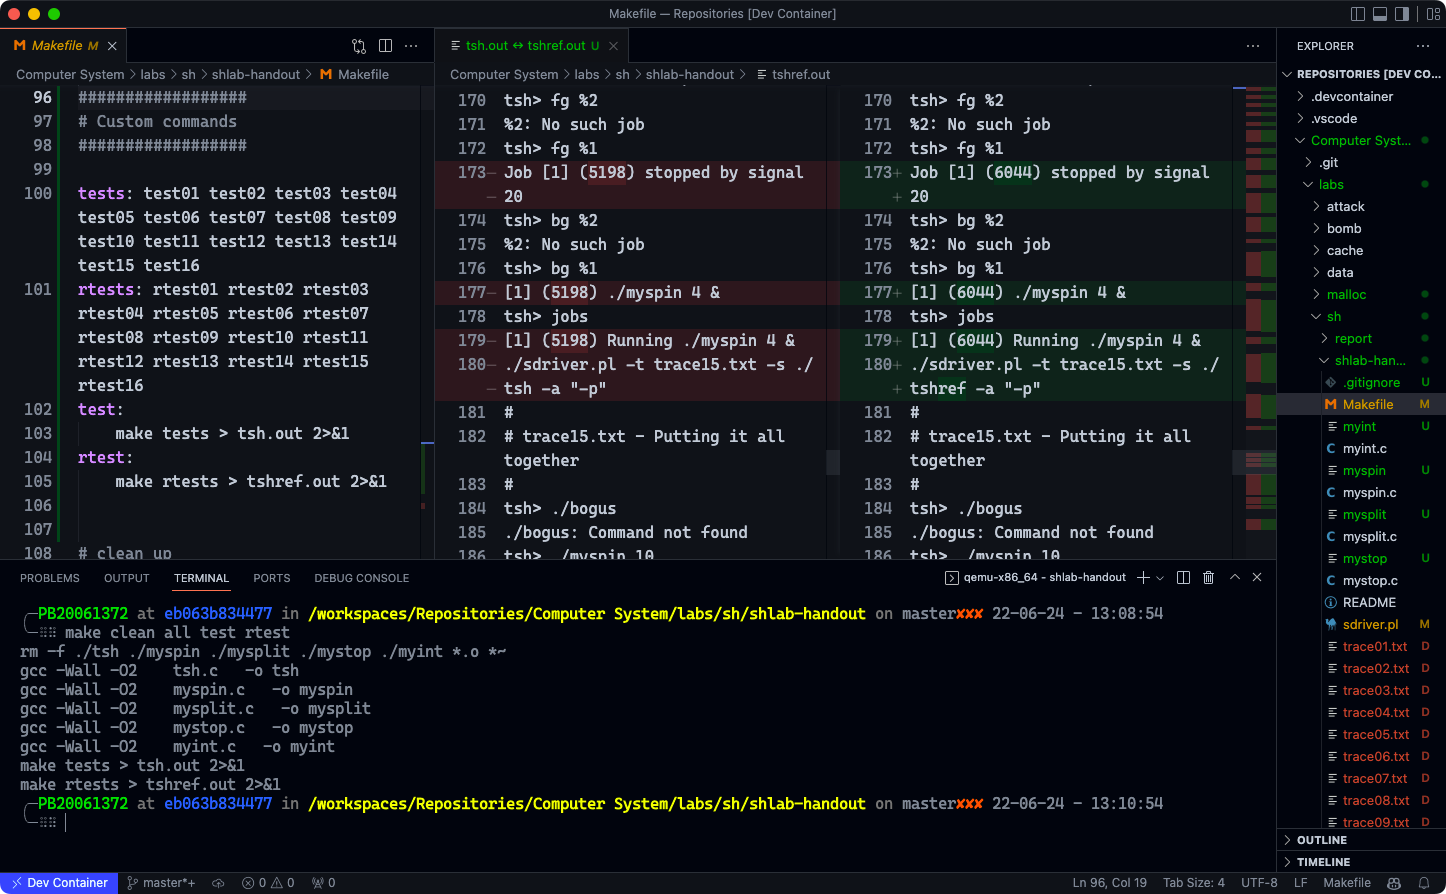
\includegraphics[width=\textwidth]{result.png}
    \caption{在Visual Studio Code中编译运行程序, 并比较输出文件}\label{result}
\end{figure}

完整源文件, 参见附录 \ref{codelist} \nameref{tsh-c}; 完整输出文件, 参见附录 \ref{outputs} \nameref{tsh-out}.

\section{实验过程}

\subsection{准备工作}

通读教材第八章 Exceptional Control Flow 与实验材料, 掌握进程控制的基本方式, 了解 \verb|waitpid|, \verb|kill|, \verb|fork|, \verb|execve|, \verb|setpgid| 和 \verb|sigprocmask| 等函数的用法. 进一步, 分析给定的框架代码 \verb|tsh.c|, 将已经实现的功能总结如下:
\begin{itemize}
    \item \verb|main| 函数: 程序初始化, 包括解析参数选项, 注册信号量处理事件等; 程序主循环, 包括读入命令行, 调用 \verb|eval| 函数等. 
    \item \verb|parseline| 函数: 解析命令行, 包括构建命令参数, 前台(foreground)或后台(background)任务的判断等.
    \item 操控任务列表的函数, 包括初始化, 添加任务, 删除任务, 查找任务, 打印任务列表等.
    \item 其他函数, 包括输出错误信息, \verb|sigaction| 函数的封装, \verb|SIGQUIT| 信号量的处理事件等.
\end{itemize}

根据 \verb|sdriver.pl| 所描述的跟踪文件格式, 对 \verb|trace01.txt| \textasciitilde\ \verb|trace16.txt| 以及参考程序输出 \verb|tshref.out| 进行分析, 将要求实现的功能总结如下:
\begin{itemize}
    \item \verb|trace01|: 读入\verb|EOF|, shell程序正常退出. 该功能已在 \verb|main| 函数主循环中实现.
    \item \verb|trace02|: 处理 \verb|quit| 命令, shell程序正常退出. 应当在 \verb|builtin_cmd| 函数中实现.
    \item \verb|trace03|: 运行一个前台任务. 相关逻辑应当在 \verb|eval| 函数实现.
    \item \verb|trace04|: 运行一个后台任务. (命令行以‘\&’字符结束.) 相关逻辑应当在 \verb|eval| 函数实现.
    \item \verb|trace05|: 处理 \verb|jobs| 命令, 打印后台任务列表. 应当在 \verb|builtin_cmd| 函数中实现.
    \item \verb|trace06| \& \verb|trace07|: 向前台任务发送 \verb|SIGINT| 信号量. 应当实现 \verb|sigint_handler| 函数.
    \item \verb|trace08|: 向前台任务发送 \verb|SIGTSTP| 信号量. 应当实现 \verb|sigtstp_handler| 函数. 
    \item \verb|trace09|: 处理 \verb|bg| 命令, 将某个停止的前台任务转移至后台运行. 应当实现 \verb|do_bgfg| 函数. 
    \item \verb|trace10|: 处理 \verb|fg| 命令, 将某个后台任务转移至前台运行. 应当实现 \verb|do_bgfg| 函数. 
    \item \verb|trace11| \textasciitilde\ \verb|trace16|: 用于验证上述功能的完整性, 包括将信号量发送至所有前台进程, 重启所有停止的进程, 错误处理, 由其他进程发送信号量等.
\end{itemize}

遵循给定框架的编码及注释风格, 补全代码, 在 Ubuntu 容器中完成所有调试. \footnote{出于简单考虑, 下文代码未实现所有错误处理的封装.} 下面, 依次解释各函数的实现方法.

\subsection{\texttt{void eval(char *cmdline)}}

该函数在主循环中调用, 输入参数为命令行字符串. 参考教材P755以及实验要求和提示, 该函数应当有如下流程:
\begin{enumerate}
  \item 调用 \verb|parseline| 函数, 解析当前命令行;
  \item 若参数列表为空, 直接返回;
  \item 调用 \verb|builtin_cmd| 函数, 若当前命令为内建命令 (\verb|quit|, \verb|jobs|, \verb|fg|, \verb|bg|), 直接处理; 否则进入下一步骤;
  \item 调用 \verb|sigprocmask| 等函数, 屏蔽 \verb|SIGCHILD| 信号量, 防止任务进程在更新任务列表前被回收(可参考教材P779);
  \item 调用 \verb|fork| 及 \verb|setpgid| 函数, 创建子进程(即任务进程), 并设置唯一的GID (等于其PID);
  \item 由于信号量屏蔽存在继承, 首先在子进程中将 \verb|SIGCHILD| 解除屏蔽; 随后调用 \verb|execve| 函数, 在子进程中运行输入的可执行目标文件(此处应有错误处理);
  \item 更新任务列表后, 在父进程(即shell进程)中将 \verb|SIGCHILD| 解除屏蔽.
  \item 若为前台任务, 调用 \verb|waitfg| 等待终止; 若为后台任务, 输出信息.
\end{enumerate}

功能完整的代码如下:
\begin{code}{c}
void eval(char *cmdline) {
  char *argv[MAXARGS]; /* argument list execve() */
  char buf[MAXLINE];   /* holds modified command line */
  int bg;              /* should the job run in bg or fg */
  pid_t pid;           /* process id */
  sigset_t mask, prev; /* signal set to block certain signals */

  strcpy(buf, cmdline);
  bg = parseline(buf, argv);
  if (argv[0] == NULL) /* ignore empty lines */
    return;

  if (!builtin_cmd(argv)) {
    sigemptyset(&mask);
    sigaddset(&mask, SIGCHLD);
    sigprocmask(SIG_BLOCK, &mask, &prev); /* block SIGCHLD */

    if ((pid = fork()) == 0) {               /* child runs user job*/
      setpgid(0, 0);                         /* set process group id */
      sigprocmask(SIG_SETMASK, &prev, NULL); /* unblock SIGCHLD in child*/
      if (execve(argv[0], argv, environ) < 0) {
        fprintf(stdout, "%s: Command not found\n", argv[0]);
        exit(1);
      }
    }

    if (!bg) {
      addjob(jobs, pid, FG, cmdline);
      sigprocmask(SIG_SETMASK, &prev, NULL); /* unblock SIGCHLD */
      waitfg(pid); /* parent waits for fg job to terminate */
    } else {
      addjob(jobs, pid, BG, cmdline);
      sigprocmask(SIG_SETMASK, &prev, NULL);
      printf("[%d] (%d) %s", pid2jid(pid), pid, cmdline);
    }
  }
}
\end{code}

\subsection{\texttt{int builtin_cmd(char **argv)}}

该函数在 \verb|eval| 中被调用, 要求实现对 \verb|quit|, \verb|jobs|, \verb|fg|, \verb|bg| 等命令的判断和直接处理, 可用简单的分支结构实现. 参考教材P755, 不难得到代码如下:
\begin{code}{c}
int builtin_cmd(char **argv) {
  if (!strcmp(argv[0], "quit")) { /* quit command */
    exit(0);
  }
  if (!strcmp(argv[0], "jobs")) { /* jobs command */
    listjobs(jobs);
    return 1;
  }
  if (!strcmp(argv[0], "bg") || !strcmp(argv[0], "fg")) { /* bf & fg command */
    do_bgfg(argv);
    return 1;
  }
  return 0; /* not a builtin command */
}
\end{code}

若为 \verb|quit| 命令, shell程序正常退出; 若为 \verb|jobs| 命令, 调用给定的 \verb|listjobs| 函数即可; 若为 \verb|fg| 或 \verb|bg| 命令, 需在 \verb|do_bgfg| 函数中处理.

\subsection{\texttt{void do_bgfg(char **argv)}}

该函数实现 \verb|fg| 或 \verb|bg| 命令的处理. 根据实验材料的描述, \verb|fg| 和 \verb|bg| 将某个任务在前台或后台重新启动, 该任务可用JID或PID指定. 此外, 为了通过跟踪文件 \verb|trace14.txt| 的测试, 需考虑若干种错误. 因此, 实现难点在于参数字符串的处理.

该程序应有如下流程:
\begin{enumerate}
  \item 若未输入参数, 报错并返回;
  \item 若参数字符串以'\%'开头, 说明输入的是JID, 否则输入的是PID;
  \item 判断输入的JID或PID是否合法(是否为数字), 若不合法, 报错并返回;
  \item 调用 \verb|getjobjid| 或 \verb|getjobpid| 函数获取目标任务的信息, 若任务不存在, 报错并返回;
  \item 调用 \verb|kill| 函数, 向目标进程组发送 \verb|SIGCONT| 信号;
  \item 修改任务状态信息. 若为前台任务, 调用 \verb|waitfg| 等待终止; 若为后台任务, 输出信息.
\end{enumerate}

完整代码如下:

\begin{code}{c}
void do_bgfg(char **argv) {
  struct job_t *job;
  int jid;
  pid_t pid;
  char *ptr;

  if (argv[1] == NULL) {
    fprintf(stdout, "%s command requires PID or %%jobid argument\n", argv[0]);
    return;
  }

  if (argv[1][0] == '%') { /* identify by JID */
    for (ptr = argv[1] + 1; *ptr; ptr++) {
      if (!isdigit(*ptr)) {
        fprintf(stdout, "%s: argument must be a PID or %%jobid\n", argv[0]);
        return;
      }
    }
    jid = atoi(argv[1] + 1);
    job = getjobjid(jobs, jid);
    if (job == NULL) {
      fprintf(stdout, "%%%d: No such job\n", jid);
      return;
    }
  } else { /* identify by PID */
    for (ptr = argv[1]; *ptr; ptr++) {
      if (!isdigit(*ptr)) {
        fprintf(stdout, "%s: argument must be a PID or %%jobid\n", argv[0]);
        return;
      }
    }
    pid = atoi(argv[1]);
    job = getjobpid(jobs, pid);
    if (job == NULL) {
      fprintf(stdout, "(%d): No such process\n", pid);
      return;
    }
  }

  kill(-(job->pid), SIGCONT); /* send SIGCONT to process group */

  if (!strcmp(argv[0], "fg")) {
    job->state = FG;
    waitfg(job->pid); /* wait for fg job to terminate */
  } else {
    job->state = BG;
    printf("[%d] (%d) %s", job->jid, job->pid, job->cmdline);
  }
  return;
}
\end{code}

\subsection{\texttt{void waitfg(pid_t pid)}}

该函数需在 \verb|eval| 及 \verb|do_bgfg| 中调用. 实现的功能为循环等待, 直至目标进程不再是前台进程(即\texttt{pid != fgpid(jobs)}). 参考程序输出显示, 等待时进程状态为 \verb|Sl+|, 故使用 \verb|sleep| 函数. 代码如下:
\begin{code}{c}
void waitfg(pid_t pid) {
  while (pid == fgpid(jobs))
    sleep(1);
  return;
}
\end{code}

\subsection{\texttt{void sigchld_handler(int sig)}}

该函数为 \verb|SIGCHLD| 的处理事件, 该信号量用于回收僵尸进程. 对于不同情形, 应输出不同提示信息, 并做相应处理. 参考教材P744 \textasciitilde\ P749以及实验材料的提示, 首先应循环调用 \texttt{waitpid(-1, \&status, WUNTRACED | WNOHANG)}, 逐个回收所有停止或终止的子进程, 进而分类讨论:
\begin{itemize}
  \item 若进程正常终止(\verb|WIFEXITED(status)|), 输出相应信息, 将该进程从任务列表中删除;
  \item 若进程接收到信号量而终止(\verb|WIFSIGNALED(status)|), 输出相应信息, 将该进程从任务列表中删除;
  \item 若进程停止(\verb|WIFSTOPPED(status)|), 输出相应信息, 将对应任务的状态修改为 \verb|ST|.
\end{itemize} 

代码如下:

\begin{code}{c}
void sigchld_handler(int sig) {
  pid_t pid;
  int status;

  while ((pid = waitpid(-1, &status, WUNTRACED | WNOHANG)) > 0) {
    if (WIFEXITED(status)) /* terminated normaly */
      deletejob(jobs, pid);
    else if (WIFSIGNALED(status)) { /* terminated by signal */
      printf("Job [%d] (%d) terminated by signal %d\n", pid2jid(pid), pid,
             WTERMSIG(status));
      deletejob(jobs, pid);
    } else if (WIFSTOPPED(status)) { /* stopped by signals */
      printf("Job [%d] (%d) stopped by signal %d\n", pid2jid(pid), pid,
             WSTOPSIG(status));
      getjobpid(jobs, pid)->state = ST;
    }
  }
  return;
}
\end{code}

\subsection{\texttt{void sigint_handler(int sig)}及\texttt{void sigtstp_handler(int sig)}}

即 \verb|SIGINT| 和 \verb|SIGTSTP| 的处理事件, 分别由 \verb|ctrl-c|, \verb|ctrl-z| 快捷键触发, 用于终止或停止前台进程. 函数体内, 应当调用 \verb|kill| 函数, 向前台任务的所有子进程发送 \verb|SIGINT| 或 \verb|SIGTSTP|. 僵尸进程的回收已经在 \verb|sigchld_handler| 函数中实现. 代码如下:

\begin{code}{c}
void sigint_handler(int sig) {
  pid_t pid = fgpid(jobs);

  if (pid != 0)
    kill(-pid, SIGINT); /* send SIGINT to foreground process group */
  return;
}
void sigtstp_handler(int sig) {
  pid_t pid = fgpid(jobs);

  if (pid != 0)
    kill(-pid, SIGTSTP); /* send SIGTSTP to foreground process group */
  return;
}
\end{code}

\clearpage
\section{总结}

完成Shell Lab, 主要有以下收获:
\begin{itemize}
    \item  掌握了系统调用, 进程控制, 信号量处理等重要的操作系统概念;
    \item  初次接触了系统级编程, 理解了通过操作系统实现应用级并发的基本方式;
    \item  实现了常用的进程控制命令, 如\verb|jobs|, \verb|bg|, \verb|fg|, \verb|quit|等, 深入理解了shell程序的原理;
    \item  熟悉了Unix系统函数库中 \verb|fork|, \verb|execve|, \verb|kill|, \verb|setpgid|, \verb|sigprocmask| 等函数的用法;
    \item  学会了封装函数用于错误处理的编程方法;
    \item  练习了Makefile的编写, 正则表达式的使用等.
\end{itemize}
本实验的所有材料已上传至GitHub:

\url{https://github.com/HasiNed/Computer-System}

\setupappendix

\clearpage
\section{部分输出结果}\label{outputs}

\subsection{\texttt{tsh.out}}\label{tsh-out}
\includecode{text}{../shlab-handout/tsh.out}

\clearpage
\subsection{\texttt{tshref.out}}\label{tshref-out}
\includecode{text}{../shlab-handout/tshref.out}

\clearpage
\section{代码清单}\label{codelist}

\subsection{\texttt{tsh.c}}\label{tsh-c}
\includecode{c}{../shlab-handout/tsh.c}

\subsection[\texttt{Makefile}]{\texttt{Makefile} (节选)}\label{makefile}
\includecode{make}{makefile.txt}

\subsection{\texttt{Dockerfile}}\label{dockerfile}
\includecode{dockerfile}{Dockerfile}